\scanpage{26}
Let $X$ be a set. A \uline{binary decomposition} of $X$ is a set of two subsets of $X$ $(\Sigma_{\alpha}^{\alpha})_{\alpha\in\unsure{\mathcal E|\mathscr E|\varepsilon}}$ (the ``hemispheres'') whose union is $X$, and of which \deleted{the intersection} neither is contained in the other -- one denotes by $E$ (``equator'') the intersection (one does not exclude its being empty). When $X$ is a topological space, one is interested in the case where the hemispheres $\Sigma_{\alpha}$ are closed, (and \inserted{in} addition, most often, \inserted{$\Sigma_{\alpha}^{\alpha}$ and $\Sigma_{\deleted{\unsure{\alpha}}}^{\alpha}\setminus E=\Sigma_{\deleted{\unsure{\alpha}}}^{\deleted{\unsure{\alpha}}\alpha,\unsure{0|\circ|o}}$} connected \deleted{\unsure{$\Sigma_{\alpha}$|the}} and where $E\ne\varnothing$); if the $\Sigma_{\deleted{\unsure{\alpha}}}^{\alpha}$ connected and $E\mathrel{\unsure{\ne|+}}\varnothing$, $X$ is connected, if \deleted{the $\Sigma_{\alpha}^{\alpha,0}$ connected}, \inserted{$X$ connected, \deleted{and}} one concludes \unsure{\deleted{immediately}} that $\overline{\Sigma^{\alpha,0}}\cap E\ne\varnothing$
% margin note written sideways
\reversemarginpar\margin{\figure{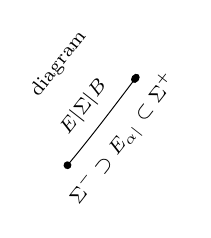
\begin{tikzpicture}[x=1mm,y=1mm,line cap=round,line join=round,font=\scriptsize]
\begin{scope}[rotate=52,transform shape]
\draw[line width=.35pt] (0,0) .. controls (4.6,-.15) and (9.5,-.08) .. (14,0);
\fill (0,0) circle[radius=.5mm];
\fill (14,0) ellipse[x radius=.64mm,y radius=.49mm];
\node[anchor=base west,inner sep=0pt] at (4.4,8.2) {diagram};
\node[inner sep=0pt] at (7.1,2.9) {$\deleted{\unsure{E|\Sigma|B}}$};
\node[inner sep=0pt] at (7,-3.6) {$\Sigma^{-}\supset E_{\unsure{\alpha|{}}}\subset\Sigma^{+}$};
\end{scope}
\end{tikzpicture}}}\normalmarginpar
(for $\overline{\Sigma^{\alpha,0}}\cap E=\overline{\Sigma^{\alpha,0}}\setminus\Sigma^{\alpha,0}$, and $\Sigma^{\alpha,0}$ cannot be both open and closed for $\Sigma^{\unsure{-,0|\alpha,0|-\alpha,0}}$, is an open set $\ne\varnothing$ and $\ne X$)

Let us consider two binary decompositions $\{\Sigma_1^{+},\Sigma_1^{-}\},\unsure{[|(}\Sigma_2^{+},\Sigma_2^{-}\}$ \deleted{\unsure{distinct}} \inserted{of $X$,} one says that they are \uline{\unsure{not mixed|not tilted|not parallel|in position}} if \inserted{they are \uline{distinct}, and if} one can find $\Sigma_1^{+}$ in one, $\Sigma_2^{+}$ in the other, such that
\[
\Sigma_1^{+}\cap\Sigma_2^{+}=\varnothing\qquad(\text{whence }E_1\cap E_2=\varnothing)
\]
one \unsure{has} then
\[
\begin{aligned}
\Sigma_1^{+}&\mathrel{\unsure{\deleted{\cap}\subset|\subset}}\Sigma_2^{-}\ \deleted{\ne\varnothing}\quad\text{i.e.}\quad\Sigma_1^{+}\cap\Sigma_2^{-}=\Sigma_1^{+}\\
\Sigma_2^{+}&\subset\Sigma_1^{-}\qquad\qquad\text{\unsure{i.e.|ie}}\quad\Sigma_2^{+}\cap\Sigma_1^{-}=\Sigma_2^{+}\\
\Sigma_{12}&\overset{\text{definition}}{=}\Sigma_1^{-}\cap\Sigma_2^{-}\supset E_1\cup E_2,\quad\Sigma_1^{-}\cap\Sigma_2^{-}\ne\varnothing
\end{aligned}
\]
% archive sheet number: 25
